
Running \ROMS on finer regional meshes with \MPAS-derived boundary conditions produces finer-scale spatial variability across the regional domains (Fig.~\ref{fig:zeta_snapshots}). The kinetic-energy records change relative to the parent and directly remapped states in a domain-dependent way (Fig.~\ref{fig:region_KE}), reflecting both the transferred state and the variability generated by the regional dynamics. Chesapeake Bay is shown separately in Fig.~\ref{fig:chesResults} because its estuarine geometry requires blending. \REVIEWc{Kyle} The figures in this subsection illustrate what the downscaled simulations produce and they clearly show that submesoscale processes are born, evolve and propagate under regional refinements, which are averaged over by the global coarse scale models. \TODOc{add more}

\begin{figure}[htbp]
\centering
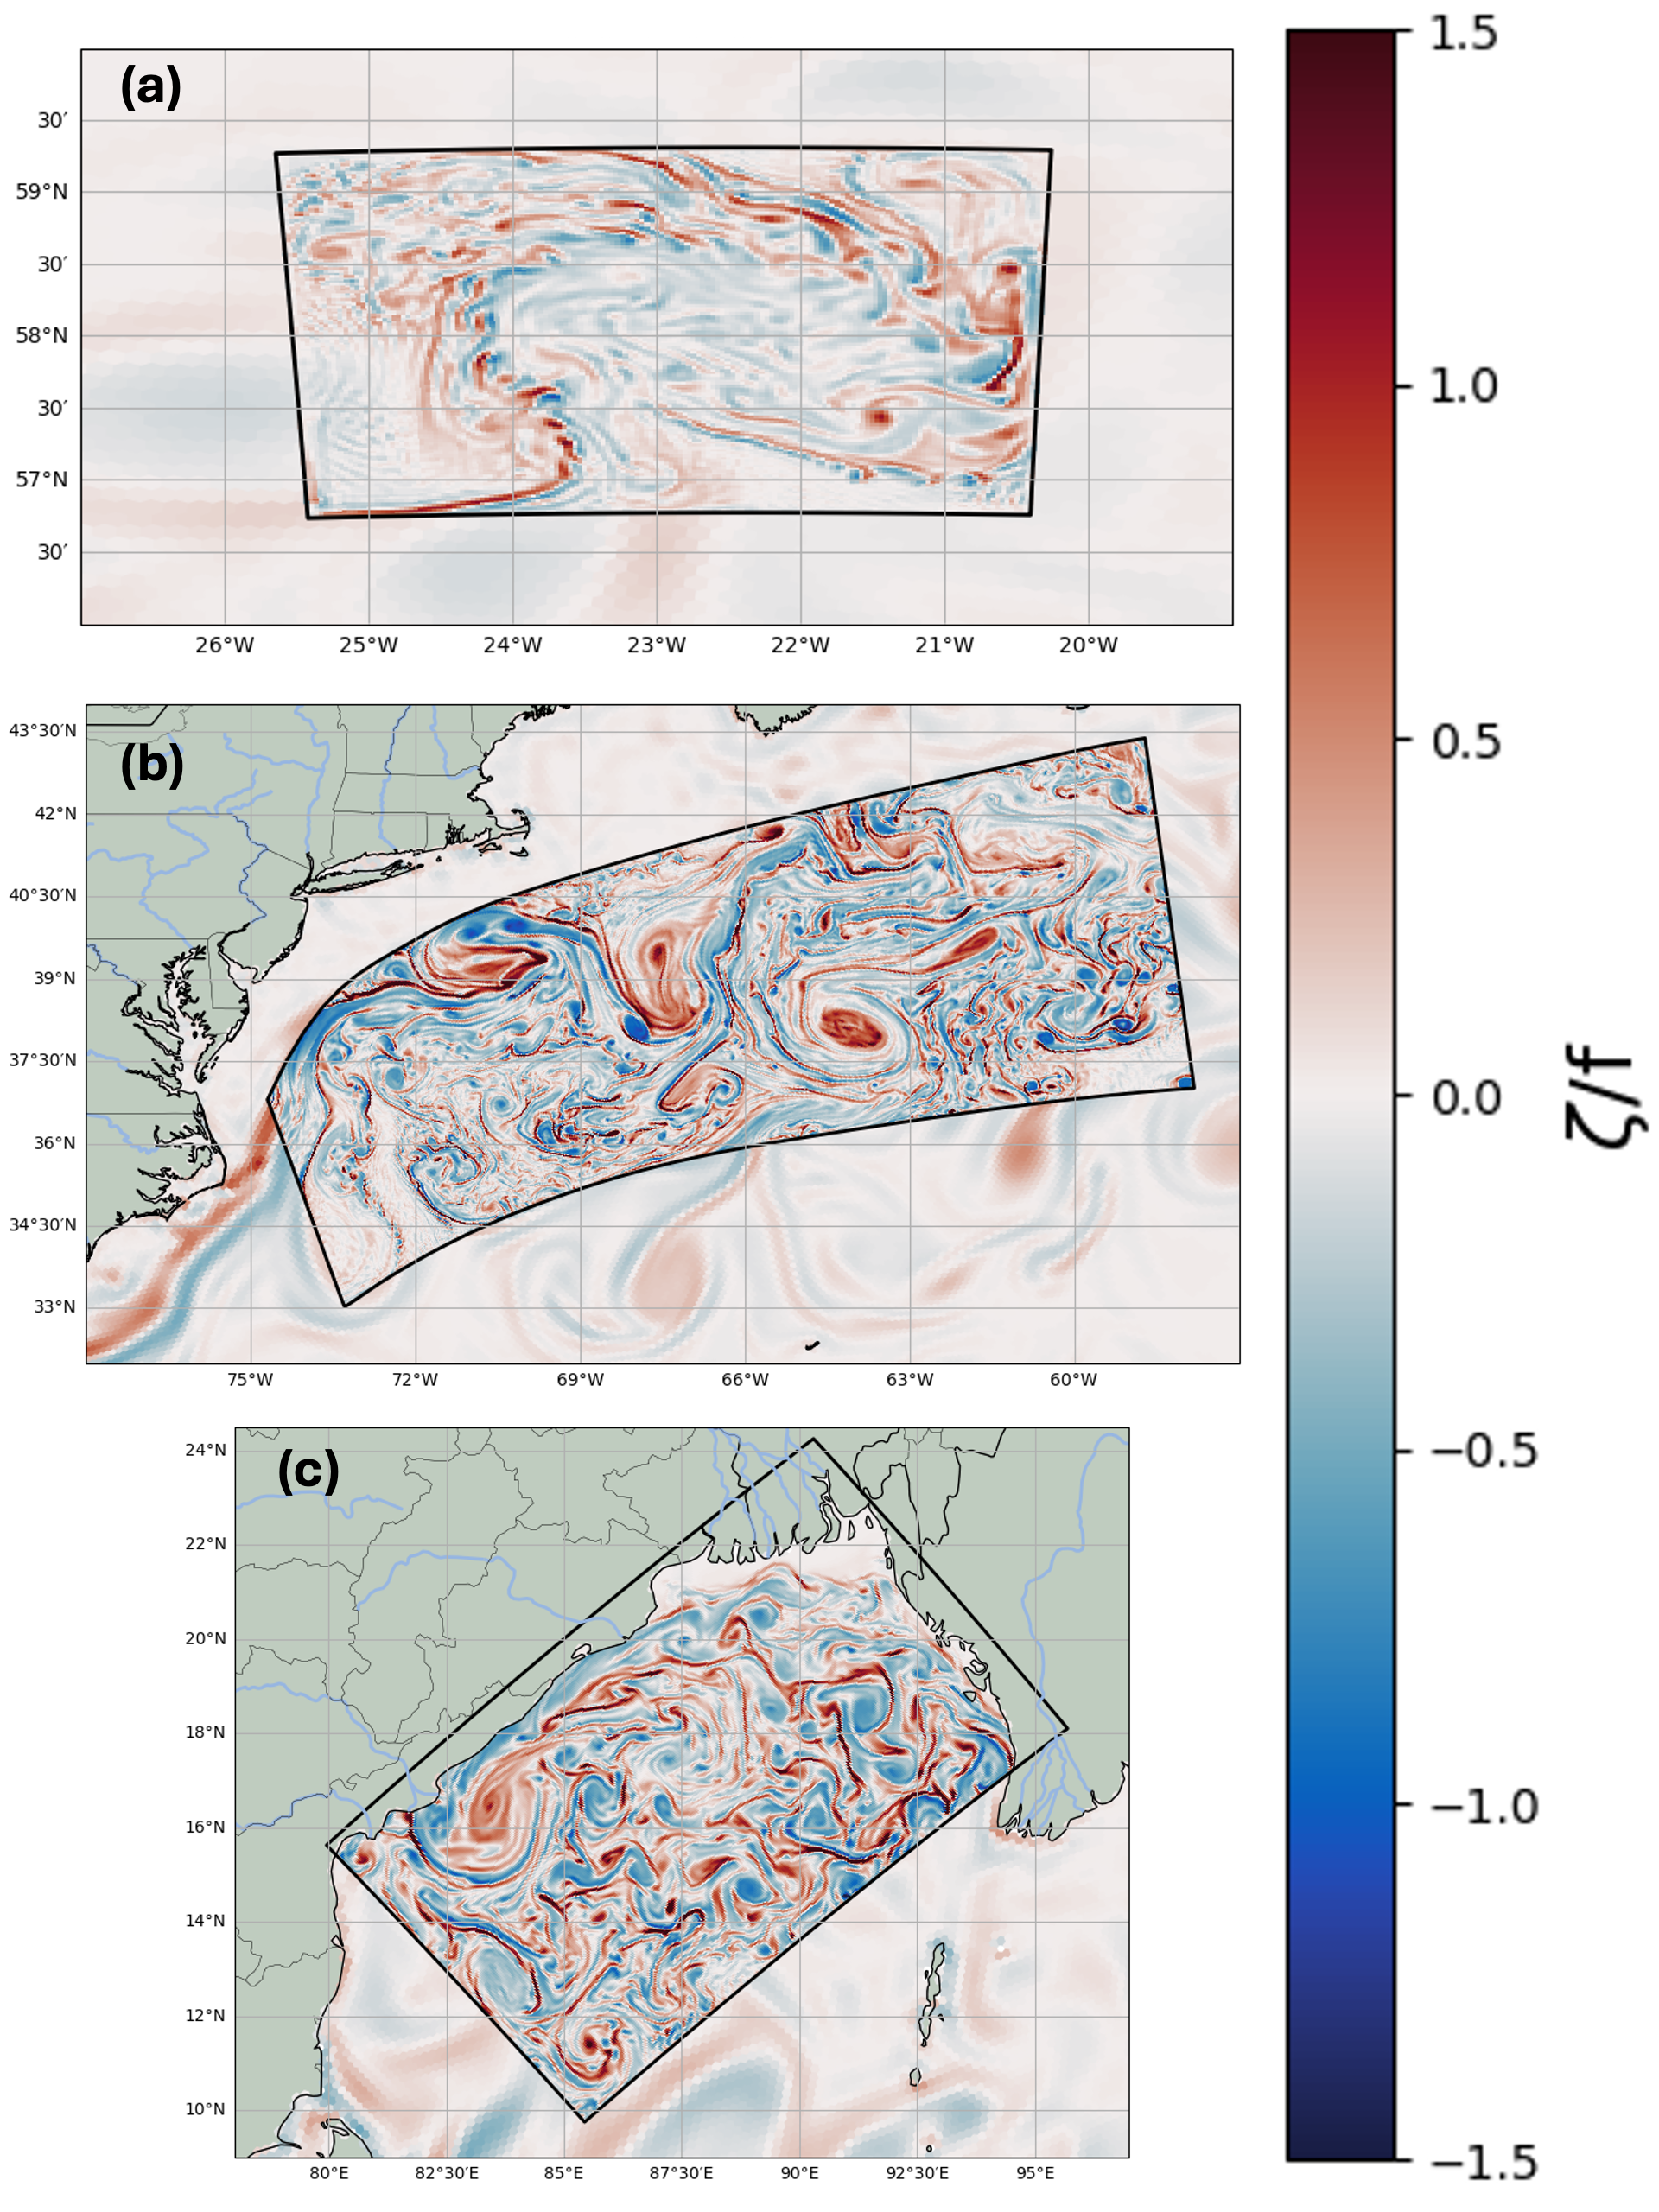
\includegraphics[width=0.90\textwidth]{Figures/zeta_3domains_v0.png}
\caption{Surface relative-vorticity fields for the North Atlantic, Gulf Stream, and Bay of Bengal regional domains.}
\label{fig:zeta_snapshots}
\end{figure}

\TODOc{Introduce and talk about benchmarks for regional domains and how these are validated}


\begin{figure}[htbp]
	\centering
	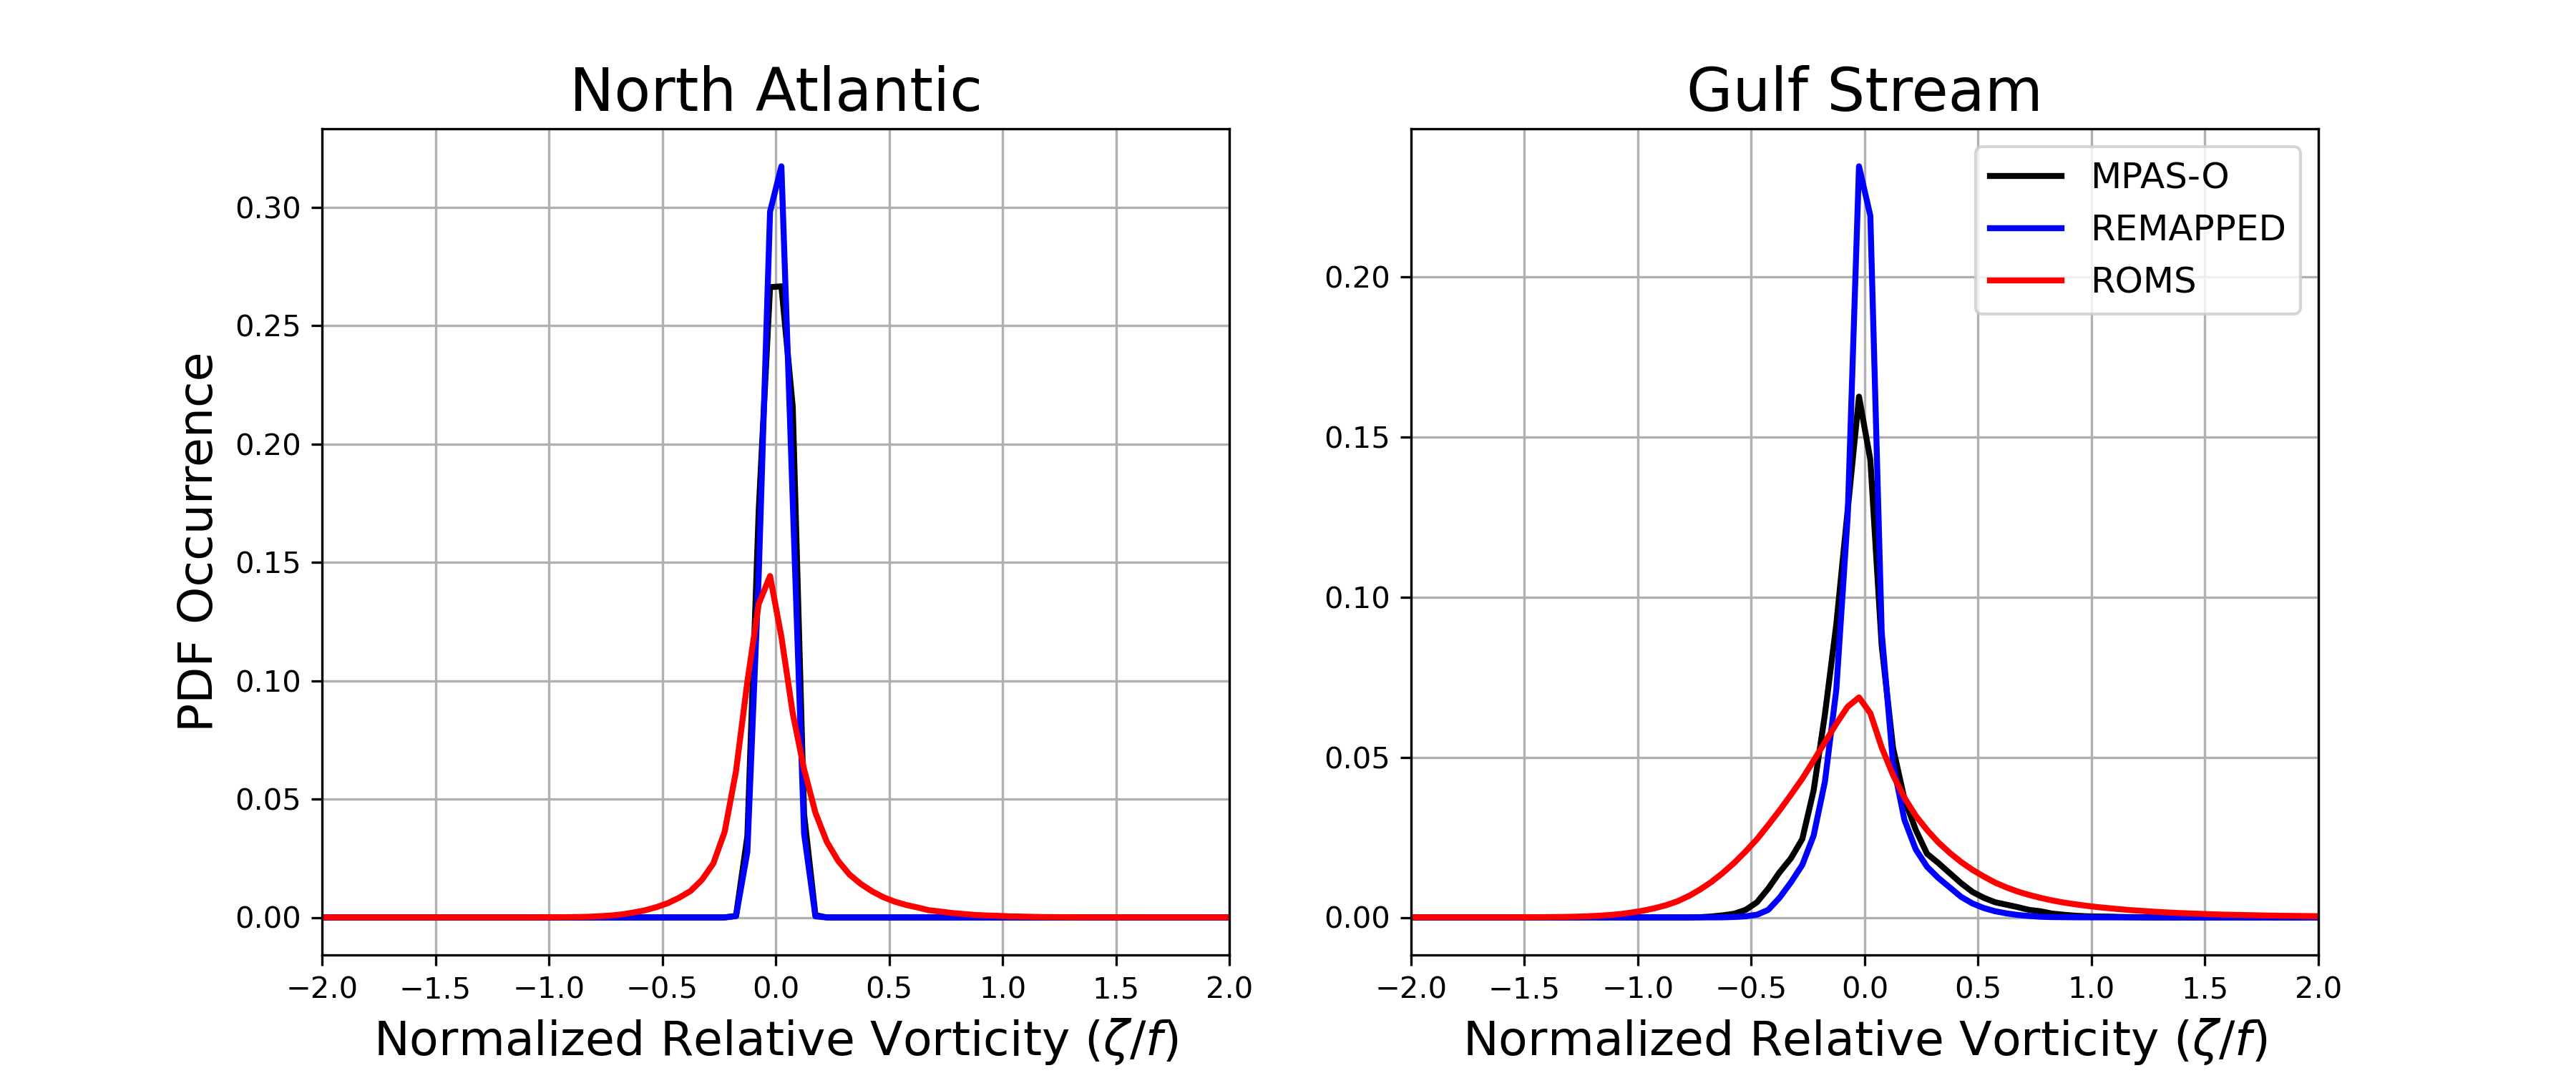
\includegraphics[width=0.88\textwidth]{Figures/regional_zeta.png}
	\caption{Normalized relative vorticity distribution for Niskine and Gulfstream cases.}
	\label{fig:relVortPDF}
\end{figure}
\FloatBarrier


The surface kinetic energy used in Fig.~\ref{fig:region_KE} is defined by
\begin{equation}
  \mathrm{KE}=\frac{1}{2}\left(u^2+v^2\right)\quad [\si{\metre\squared\per\second\squared}],
  \label{conv:eq:ke}
\end{equation}
with velocities represented at cell centers for the diagnostic.

\begin{figure}[htbp]
\centering
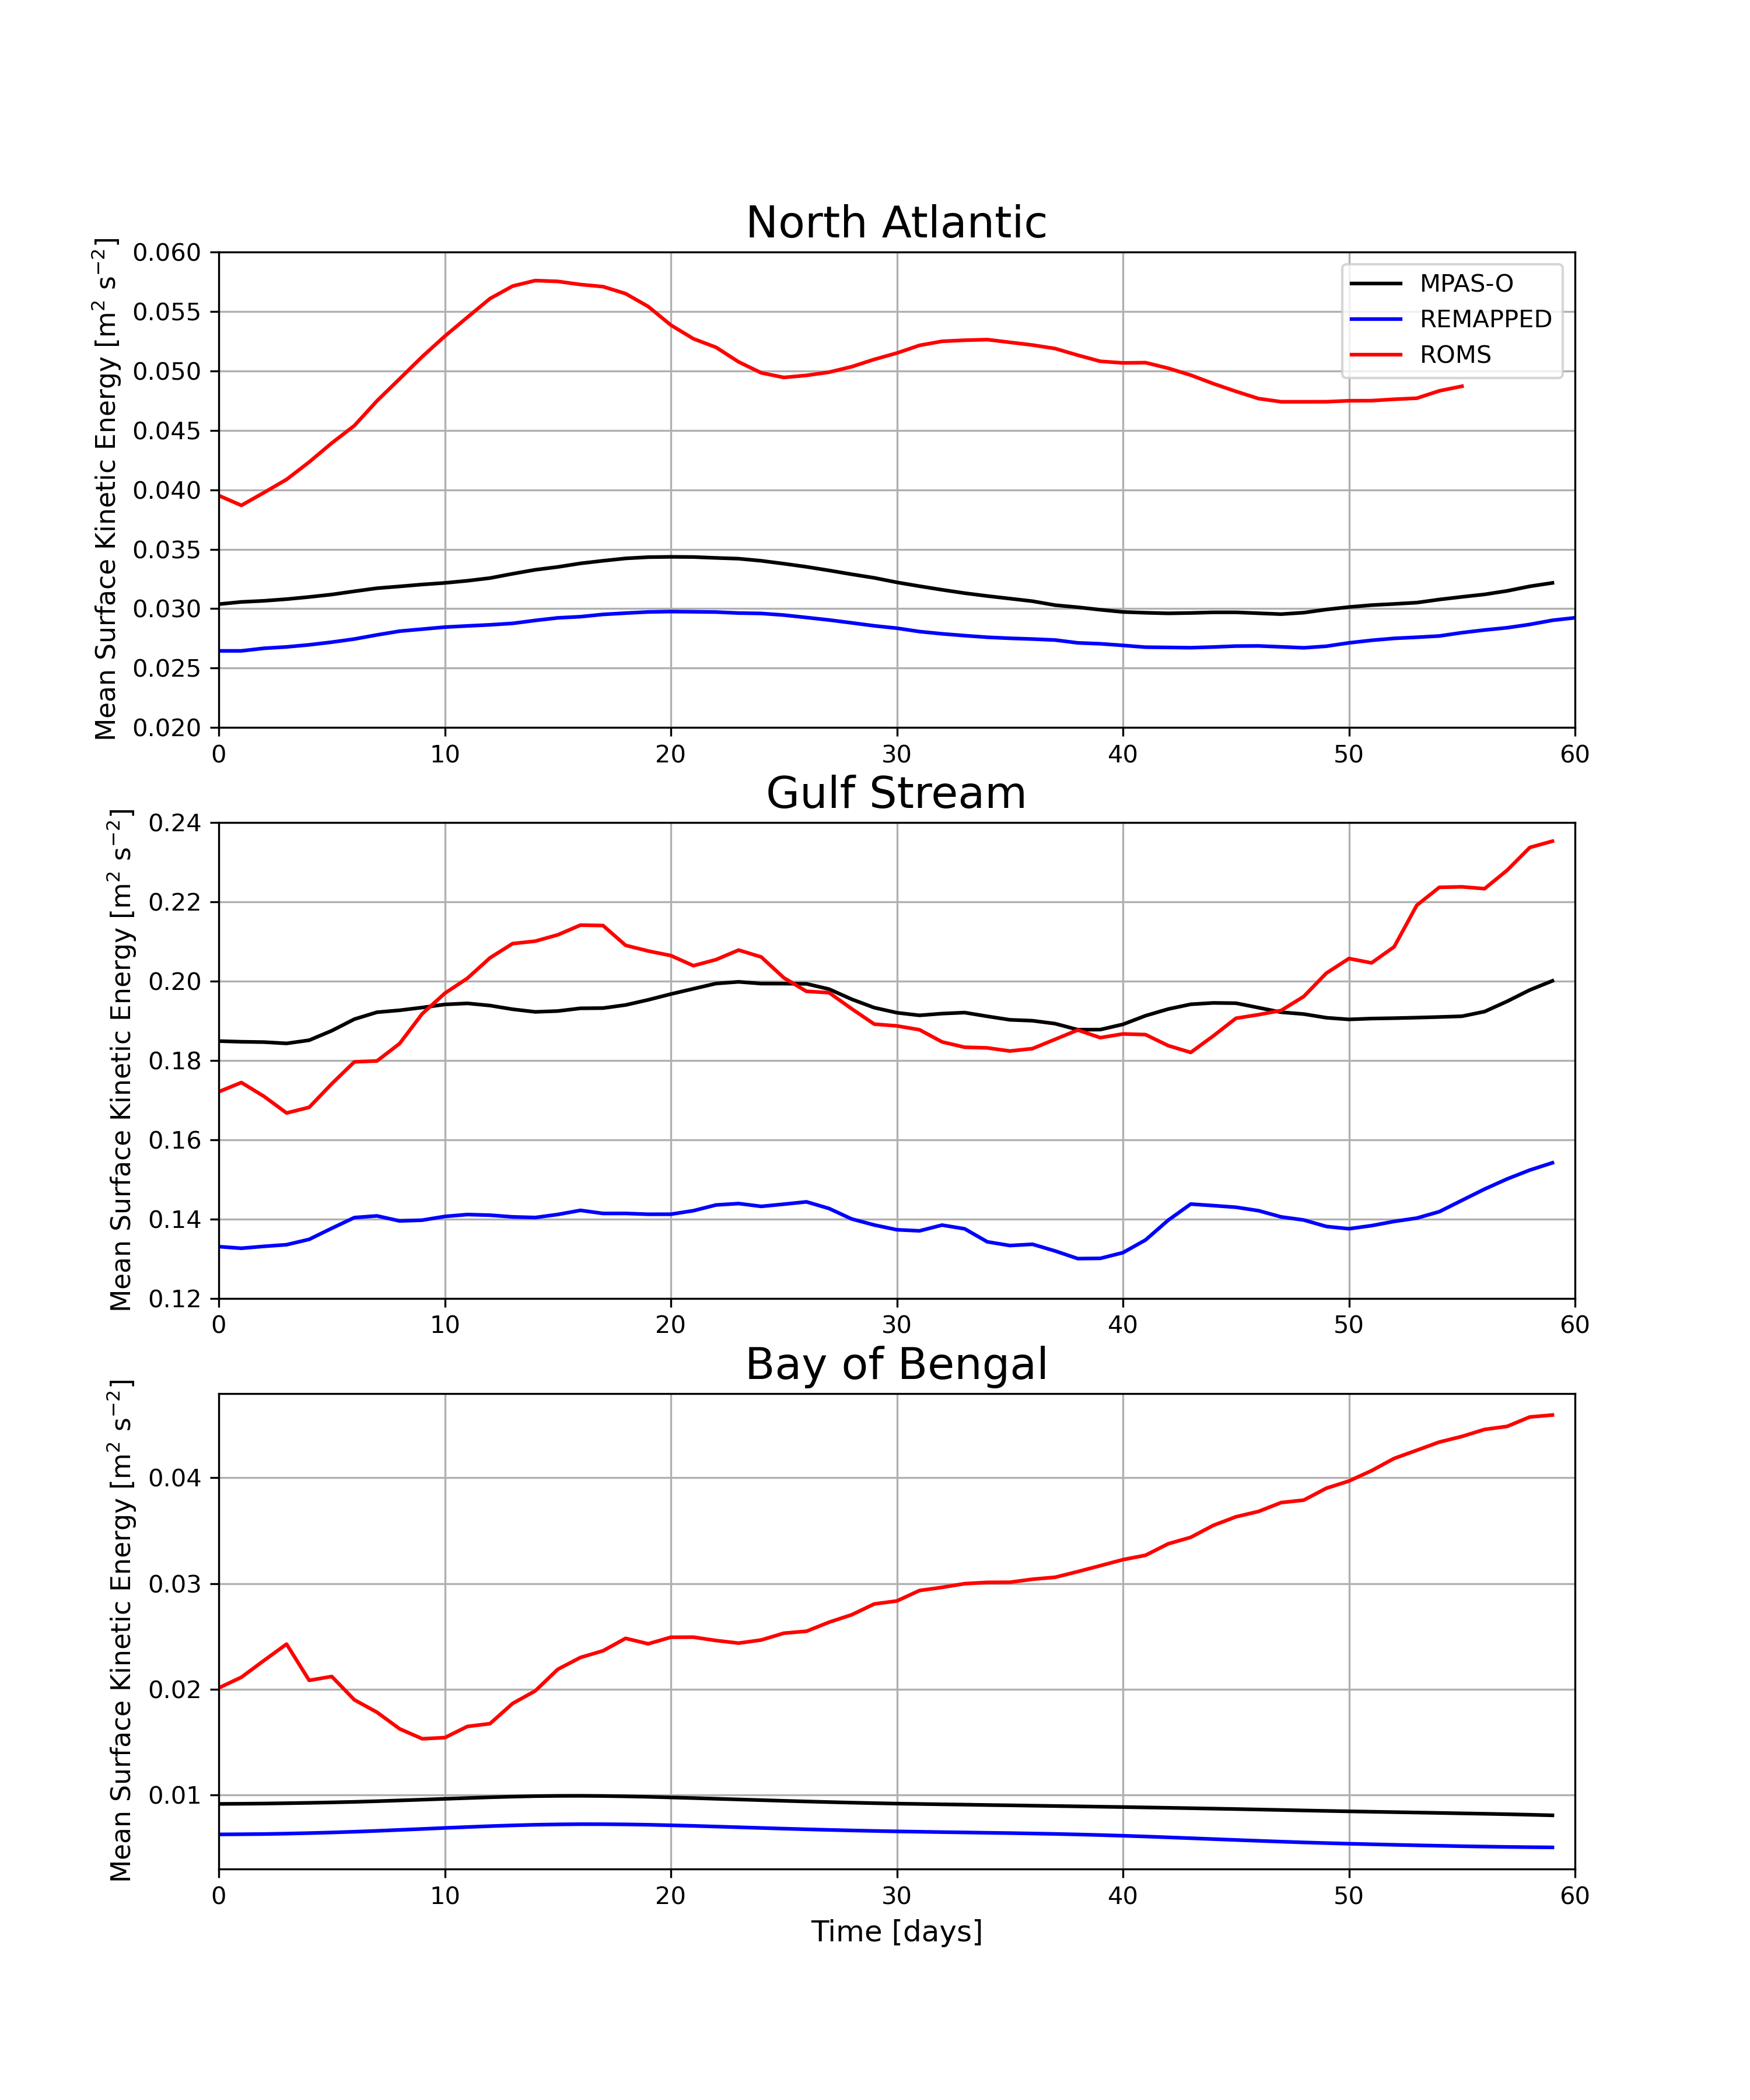
\includegraphics[width=\textwidth]{Figures/Region_KE_TimeSeries_3domains.png}
\caption{Surface specific kinetic-energy time series for the North Atlantic, Gulf Stream, and Bay of Bengal domains, evaluated with the diagnostic definition in Eq.~\eqref{conv:eq:ke}.}
\label{fig:region_KE}
\end{figure}

\begin{figure}[htbp]
\centering
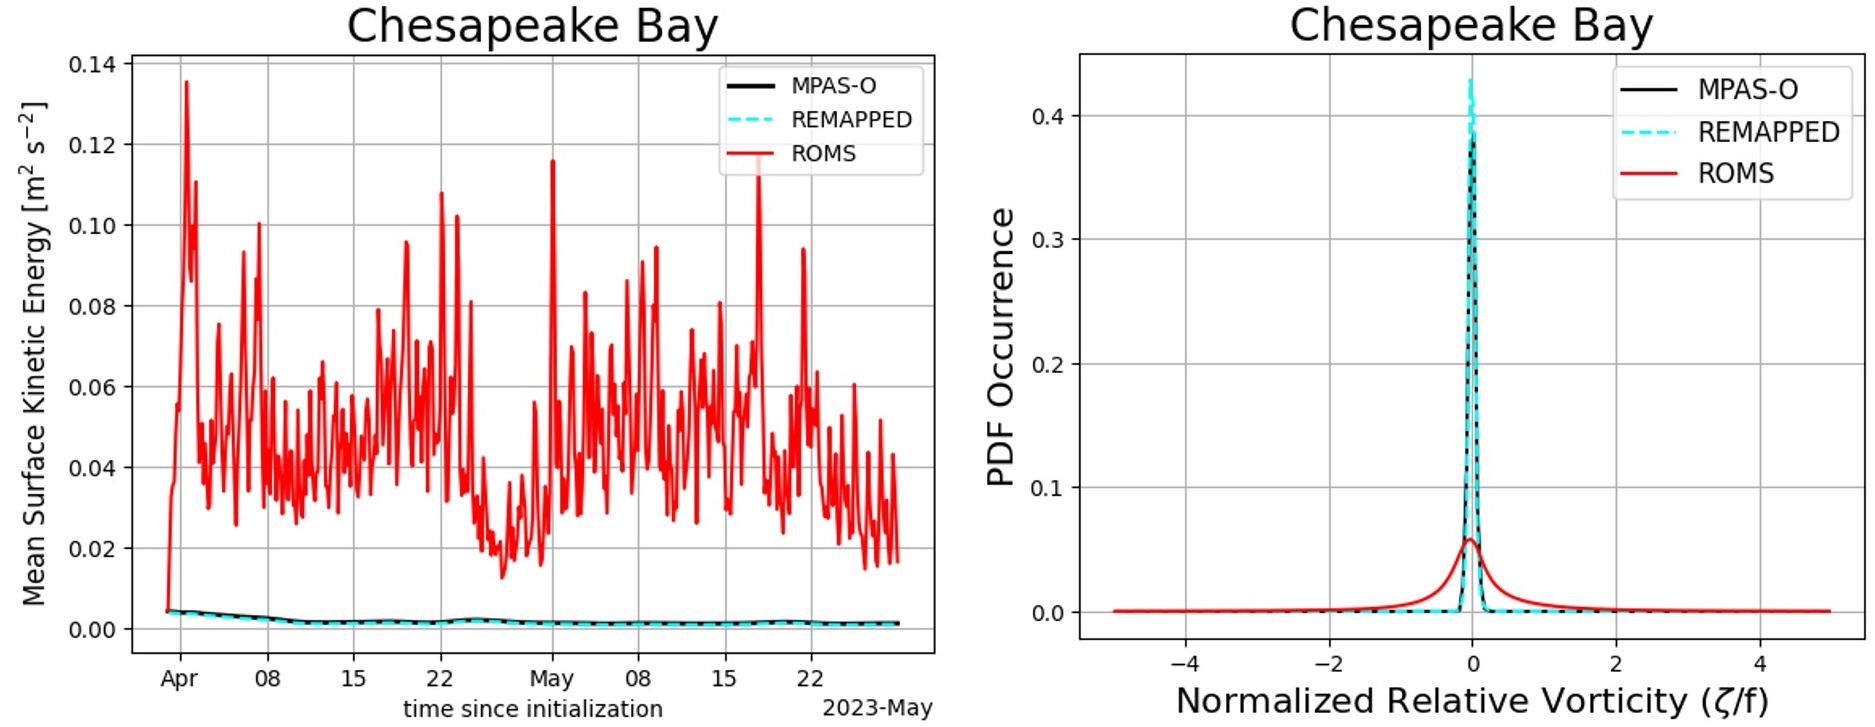
\includegraphics[width=0.88\textwidth]{Figures/chesbay_ke_zeta.jpg}
\caption{Surface specific kinetic energy and relative-vorticity distribution for Chesapeake Bay. These estuarine results are preliminary.}
\label{fig:chesResults}
\end{figure}
\FloatBarrier

The open-ocean and coastal applications occupy relative target scales near $\hRatio\approx0.2$--$0.35$, whereas Chesapeake Bay is substantially finer relative to its parent. In every domain the regional solution alters both the geometry of the flow and its energy content relative to the parent state. Because the regional model continues to evolve after initialization, these differences measure the combined effect of the transfer and the subsequent regional dynamics, and the convergence experiments of Sect.~\ref{conv:sec:conv} remain the quantitative statement about the transfer itself. The Chesapeake result depends particularly strongly on native bathymetry, land-mask treatment, and the blended estuarine fields. \TODOc{talk more about practical implementation of this case}
